\chapter{Implementação}
A implementação do sistema segue todas as diretrizes de tecnologias e conceitos apresentados até este tópico. A descrição de como a implementação foi feita será dividida em duas partes principais: \textit{backend} e \textit{frontend}. Sendo a parte de \textit{backend} a implementação da infraestrutura e servidor da aplicação, e na parte do \textit{frontend} a implementação de interface com o usuário. No desenvolvimento elegemos um nome fictício para a aplicação, chamado Orb. Este nome será utilizado para remeter a aplicação em alguns textos, logos, implementações, entre outros.

O código-fonte da aplicação está hospedado no GitHub \cite{orb}, como \textit{software open-source}, liberado para utilização através da licença MIT \cite{mit}. A abordagem utilizada para a descrição da implementação feita fará referências pontuais a trechos do código-fonte que poderão ser consultados pelo leitor no repositório informado \cite{orb}, evitando-se ao máximo a exposição de código neste formato de texto que não é favorável a análise deste tipo de conteúdo.

\section{Backend}
Primeiramente iremos descrever a criação do ambiente de desenvolvimento do projeto, onde inicialmente foi instalado o sistema operacional e todas as ferramentas que decidimos utilizar para a construção da aplicação, e posteriormente iniciamos o processo de codificação.

Iniciando-se pelo sistema operacional, foi criada uma partição separada no disco rígido do computar que dispúnhamos, com volume de 60 GBs. O sistema operacinal escolhido para o ambiente de desenvolvimento foi de uma distribuição Linux chamada CentOS \cite{centos}, versão 7. A instalação do sistema operacional foi feita através de um \textit{pendrive} e foram seguidas todas as configurações padrões do \textit{wizard} de instalação do sistema.

Após a instalação do sistema operacional, fizemos a instalação de todas as ferramentas, a nível de O.S., que foram escolhidas para o desenvolvimento da aplicação, como o NodeJS, MongoDB, Redis, editores de texto e navegadores. Todas estas ferramentas foram instaladas através do repositório de pacotes padrão do sistema CentOS 7, chamado YUM. Para algumas ferramentas foram necessário a atualização das fontes do repositório YUM e outras foram instaladas através de pacotes RPM disponibilizados no próprio site da ferramenta.

A implementação do \textit{backend} iniciou-se com a criação de um diretório chamado backend na pasta raiz do projeto, do qual a partir dele foram seguidas recomendações de boas práticas \cite{express-app-structure} para a organização da estrutura de diretórios em aplicações ExpressJS. A seguinte listagem identifica o nome destes diretórios e suas respectivas funcionalidades:

\begin{description}
	\item[controllers] Este diretório contém os arquivos de código relacionados as rotas e suas lógicas de implementação. Rotas são os \textit{endpoints} que podem ser acessados através de requisições HTTP enviadas por uma determinada URL que a identifica. Neste diretório contém os arquivos das rotas de cliente, usuário e \textit{token}.
	
	\item[domain] Este diretório contém os arquivos relacionados a lógica de negócio da aplicação. Os \textit{handlers} que tratam as requisições \textit{websocket} da aplicação estão implementados em arquivos contidos nesta pasta.
	
	\item[helpers] Este diretório contém arquivos que implementam funcionalidades que podem ser utilizadas em diversos pontos do sistema, este diretório funciona como um \textit{cross-cutting layer} da aplicação. Nesta pasta estão implementados alguns métodos que ajudam na geração de \textit{random strings} e retorno de \textit{datetime} em formato UTC.
	
	\item[middlewares] Este diretório contém arquivos relacionados a \textit{middlewares} de tratamento de requisições que chegam ao servidor, como realização de autenticação e autorização de acesso as rotas da aplicação.
	
	\item[models] Este diretório contém arquivos relacionados aos objetos que podem ser persistidos na aplicação. Devido ao Javascript ser uma linguagem dinâmica, estes objetos não representam um contrato de como estes eles devem existir na aplicação, mas como eles devem ser persistidos no banco de dados, que no caso desta aplicação é o MongoDB. Neste diretório serão encontrados os arquivos de persistência dos \textit{tokens}, \textit{chat}, \textit{messages}, \textit{users}, entre outros.
\end{description}

Após a definição da estrutura de diretórios da aplicação, foi realizada a instalação e inicialização do NPM, responsável por gerenciar todos os pacotes que iremos utilizar no desenvolvimento da solução.

\subsection{Persistência}
A persistência dos dados foi feita em um banco de dados MongoDB, onde para sua utilização foi feito o \textit{download} doo pacote Mongoose pelo NPM. A conexão com o banco foi feita no arquivo de inicialização da aplicação, através do método connect do próprio Mongoose, passando-se como parâmetros uma \textit{connection string} com o endereço local do banco de dados. Por ser um ambiente de testes, não utilizamos autenticação com o banco de dados, mas caso fosse necessário, bastava-se apenas adicionar os dados de \textit{username:password} na própria \textit{connection string}.

No diretório \textit{models} foram criados arquivos para cada objeto que fosse ser persistido no banco. As implementações da persistência utilizaram o Mongoose como modelo, exportando de cada módulo o objeto \textit{schema} de cada persistência, podendo através deste realizar todas as operações de CRUD.

A seguinte imagem ilustra a representação dos objetos persistidos no banco de dados:

\begin{figure}[!htb]
	\centering
	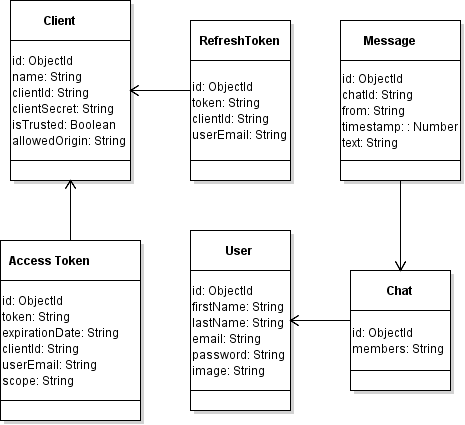
\includegraphics[scale=0.85]{imagens/models_uml.png}
	\caption{\small Representação UML dos modelos persistidos no banco de dados.}
	\label{fig:modelsuml}
\end{figure}


\subsection{Autenticação e Autorização}
Para a implementação do sistema de autenticação, cujos códigos estão no diretório middlewares, utilizamos três pacotes NPM, que funcionam como \textit{middlewares} que extraem de um \textit{request} as informações de autenticação, e através de uma \textit{callback} é possível validar essas informações e sinalizar se as informações estão corretas para concretização da autenticação. Para o sistema de autorização, utilizamos o OAuth2 com algumas modificações em seu padrão para atender aplicações \textit{trusted}, como o nosso \textit{frontend app} desenvolvido em AngularJS, que é um tipo de aplicação que não necessita de autorização do usuário da conta para acessar suas informações confidenciais.

Como estamos utilizando um sistema de \textit{tokens}, para realizar acesso ao \textit{endpoint} token, o qual é utilizado no sistema de \textit{login} para se conseguir um Access Token e um Refresh Token através do fornecimento de \textit{e-mail} e senha, é realizada a autenticação pelos padrões Basic \cite{passport-basic} e Client \cite{passport-client}. Após esta autenticação, o usuário é encaminhado para um \textit{exchange} do OAuth2 que irá gerar, persistir e retornar um Access Token e um Refresh Token para o solicitante, que poderá usá-lo para acessar os demais \textit{endpoints} da aplicação.

Como já introduzido, o restante dos das rotas da aplicação são protegidos através do padrão de autenticação Bearer \cite{passport-bearer}, que procura em cada requisição feita um Access Token, que será verificado, e caso seja válido permitirá o acesso ao \textit{endpoint} solicitado. Em caso do Access Token não ser válido, o servidor irá emitir uma resposta de erro, HTTP 401, informando o problema ocorrido, e se o problema for a expiração do Access Token, ele poderá utilizar o Refresh Token para conseguir um novo Access Token válido por mais um determinado tempo, evitando de ter que realizar toda o processo de autenticação com \textit{e-mail} e senha novamente.

\begin{figure}[!htb]
	\centering
	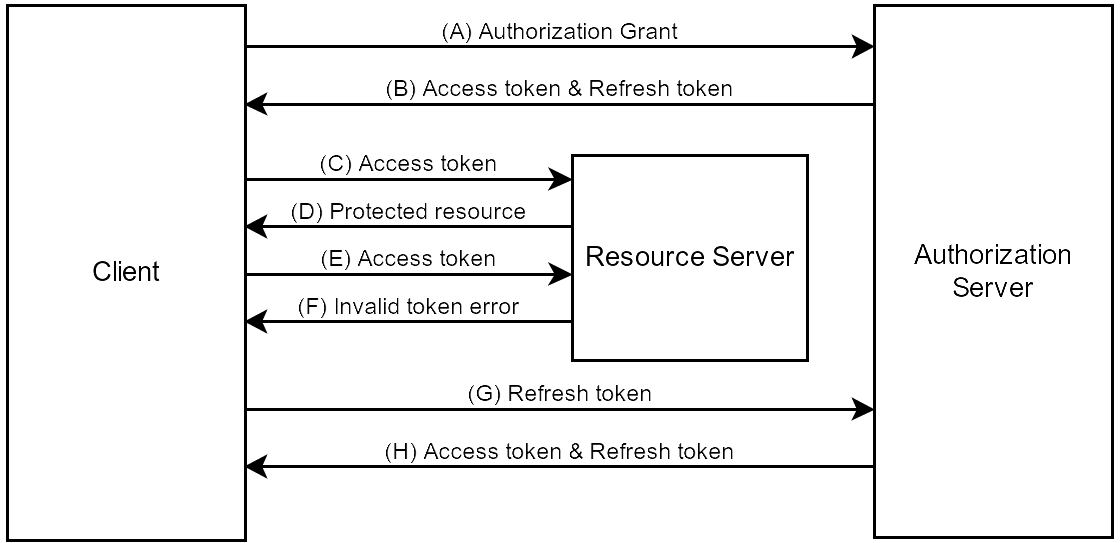
\includegraphics[scale=0.49]{imagens/oauth2.png}
	\caption{\small Fluxo de acesso aos recursos com OAuth2. Fonte: jlabusch \cite{img-jlabusch}}
	\label{fig:oauth2}
\end{figure}

\subsection{Rotas}


\subsection{Socket}


\section{Frontend}

